\chapter{Результаты численного моделирования}

\section{Проверка адекватности модели дыхательной системы при расчете альвеолярных вентиляции и давления}
Константы и параметры модели дыхательной системы показаны в \ref{tab:langPuram}, \ref{tab:lang1d}. 
Они были идентифицированы в соответствии с анатомическими CT данными, литературными данными \cite{bental2013,Simakov2009,Mead1961} и результатов сравнения модели с данными из \cite{schmidt}.  большинство параметров легочной вентиляции на альвеолярный газообмен, альвеолярный поток воздуха и альвеолярное давление. В данном численном эксперименте был выполнен расчет динамики изменения общей альвеолярной вентиляции и альвеолярного давления. Результаты моделирования показаны на рисунках \ref{image4}, \ref{image5}. Рассчитанные значения (на графике обозначены точками) сравнивались с литературными данными из \cite{schmidt} (на графике обозначены сплошными линиями)  Из построенных графиков видно, что достигнуто хорошее соответствие численных и экспериментальных результатов.

\begin{figure}[!ht]
	\centering
	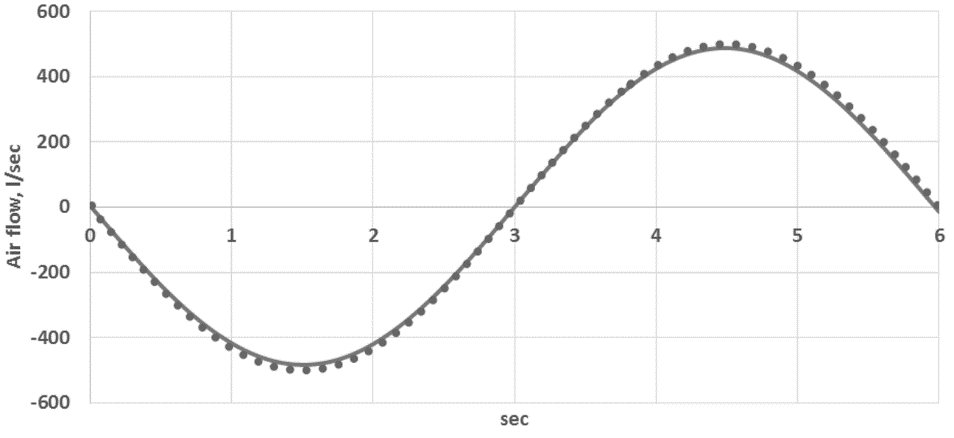
\includegraphics[scale=1.5]{image4}
	\caption{Сравнение расчетных и экспериментальных данных по альвеолярной вентиляции (лит/сек): сплошная линия --- данные из \cite{schmidt}, точки --- численный расчет.} 
	\label{image4}	
\end{figure}

\begin{figure}[!ht]
	\centering
	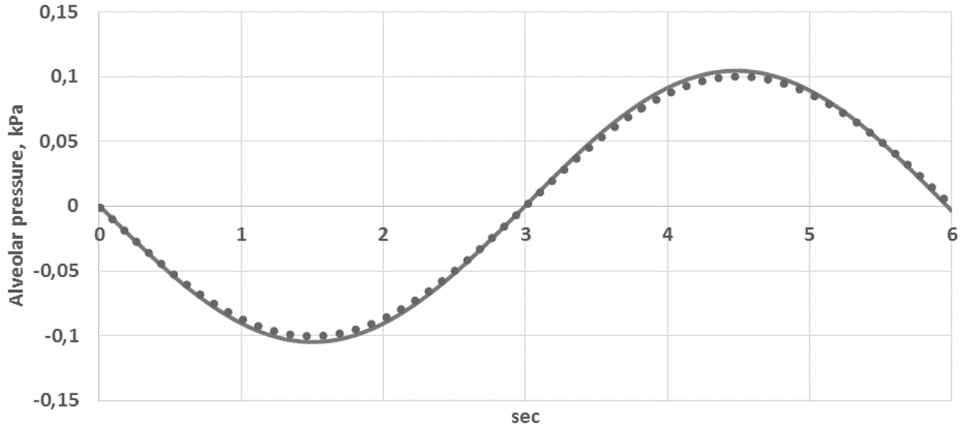
\includegraphics[scale=1.5]{image5}
	\caption{Сравнение расчетных и экспериментальных данных по альвеолярному давлению (кПа): --- данные из \cite{schmidt}, точки --- численный расчет} 
	\label{image5}
\end{figure}


\section{ Эффективность выведения углекислого газа из организма при искусственной вентиляции легких}

Искусственная вентиляция легких широко используется в хирургии для поддержания необходимых процессов жизнедеятельности при анестезии. В настоящее время параметры искусственной вентиляции (дыхательный объем и чистота дыхания) корректируются в ручном режиме анестезиологом на основе жизненных показателей пациента.  Основная задача анестезиолога поддерживать основные функции организма с помощью достаточной поставки $O_{2} $ и выведения излишка $CO_{2} $ через легкие. Определенные физиологические показатели непосредственно не анализируются и не контролируются во время анестезии, например концентрация $CO_{2} $ в артериальной крови. Понимание взаимосвязи между параметрами искусственной вентиляцией и альвеолярной концентрацией $O_{2} $ и $CO_{2} $ очень важно для дальнейшего ойенивания возможности выведения излишков $CO_{2} $ с помощью вентиляции легких. 

В данном разделе с помощью численной модели дыхательной системы выполнено изучение зависимости альвеолярной концентрации $CO_{2} $ от частоты дыхательных циклов. При моделировании использовались следующие предположения. Минутная вентиляция $\left(V_{{\rm minute}}\right)$ считалась фиксированной, а дыхательный объем $\left(V_{td} \right)$ рассчитывался из уравнения:
\begin{equation} \label{GrindEQ__38_} 
60V_{td} \nu _{ARR} =V_{minute} =const 
\end{equation} 
Плевральной давление в уравнении \eqref{GrindEQ__10_} было "выключено" $\left(p_{g} =0\right)$ и давление на входе в носоглотку в уравнении \eqref{GrindEQ__6_} описывалось по закону:
\begin{equation} \label{GrindEQ__39_} 
S_{1} \left(t,0\right)u_{1} \left(t,0\right)=Q_{td} \sin \left(2\pi \nu _{ARR} t\right),\; Q_{td} ={V_{td} \mathord{\left/ {\vphantom {V_{td}  \int _{0}^{{T\mathord{\left/ {\vphantom {T 2}} \right. \kern-\nulldelimiterspace} 2} }\sin \left(2\pi \nu _{ARR} t\right) }} \right. \kern-\nulldelimiterspace} \int _{0}^{{T\mathord{\left/ {\vphantom {T 2}} \right. \kern-\nulldelimiterspace} 2} }\sin \left(2\pi \nu _{ARR} t\right) } dt=\frac{V_{td} }{\pi \nu _{ARR} } ,  
\end{equation} 
где $\nu _{ARR} $ чистота искусственной вентиляции (ARR), $Q_{td} $ амплитуда ингалируемого потока воздуха. Величина частоты вентиляции изменялась в допустимых физиологических пределах $\left(0<\nu _{ARR} <0.7\; Hz\right)$. Величина концентрации $CO_{2} $ в альвеолярном объемы была получена на основе комплексной модели описанной в разделе \ref{chapter:lungs} и осреднении значений по нескольким дыхательным циклам искусственной вентиляции.  Результаты моделирования показаны на рисунке \ref{opt}.

\begin{figure}[!ht]
	\centering
	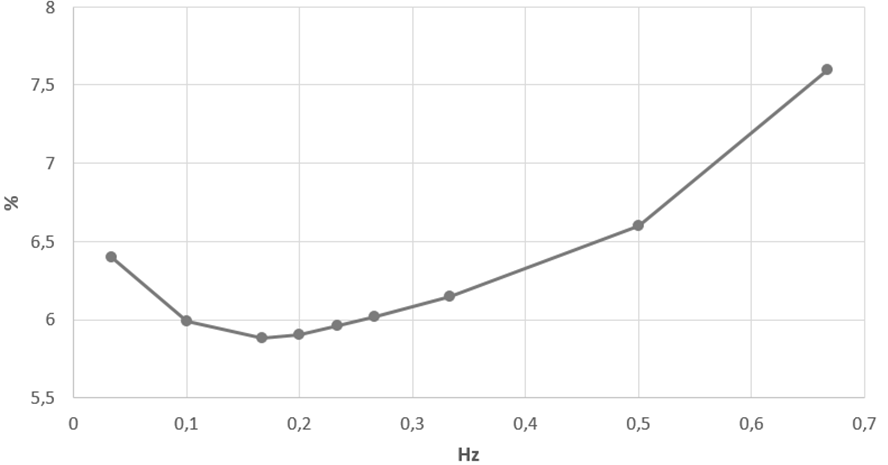
\includegraphics[scale=0.75]{opt}
	\caption{Альвеолярная концентрация $CO_{2} $} 
	\label{opt}
\end{figure}

Минимизация значения концентрации $CO_{2} $ рассматривалась как критерий эффективности функционирования легких при проведении искусственно вентиляции. Начальное увеличение чистоты вентиляции от нуля приводит к увеличению выведения $CO_{2} $ из организма и уменьшению альвеолярной концентрации $CO_{2} $  Минимальное значение концентрации было достигнуто при чистоте вентиляции \textit{0.17~Hz}, полученное значение находится достаточно близко к экспериментально измеренной величине чистоты дыхания пациента в обычном состоянии(\textit{0.23~Hz}). Дальнейшее увеличение чистоты вентиляции приводит к увеличению концентрации  $CO_{2} $. Таким образом, углубленное дыхание позволяет поддерживать требуемую альвеолярную вентиляцию за счет уменьшения доли мертвого пространства в дыхательном объеме. Однако, глубокие вдохи сопряжены с увеличением эластичного сопротивления. С другой стороны, при частом поверхностном дыхании, помимо ухудшения условий газообмена из-за большой доли мертвого пространства в дыхательном объеме, повышается неэластическое сопротивление благодаря ускорению ин- и экспираторных потоков в воздухоносных путях. Энергетически оптимальным оказывается некий средний по своим параметрам паттерн дыхания, неодинаковый для разных людей. Установлено, что любой человек при свободном дыхании избирает обычно именно такой паттерн, соответствующий минимуму энергозатрат на работу дыхания и отражающий морфологические и функциональные особенности того или иного организма. В результатов численного эксперимента следует, что чистота искусственной вентиляции должны быть достаточно близка к значению чистоты дыхания пациента в обычном состоянии.  

\section{Моделирование альвеолярного газообмена при патологических рисунках дыхания}
Рисунок дыхания является важной характеристикой дыхательной системы, который заметно влияет на эффективность альвеолярного газообмена. Патологическое (периодическое) дыхание -  внешнее дыхание, которое характеризуется групповым ритмом, нередко чередующимся с остановками или со вставочными периодическими вдохами. 

В данной работе рисунок дыхания определятся определяется временным профилем плеврального давления (функция $p_{pl} \left(t\right)$ в уравнении \eqref{GrindEQ__10_}. В данном разделе выполнено численное исследование зависимости альвеолярной концентрации $CO_{2} $ и $O_{2} $ от рисунка дыхания. Рассмотрено два патологических типа дыхания: Биота и Чейна-Стокса \cite{Wijdicks2007,Pearce2002}, а также выполнено сравнение с нормальным(синусоидальным) дыханием \cite{schmidt}. Нормальное дыхание моделировалось с помощью условия:
\begin{equation} \label{GrindEQ__40_} 
p_{pl} \left(t\right)=p_{g} \sin \left(vt\right).  
\end{equation}

Дыхание Биота - форма периодического дыхания, характеризующаяся чередованием равномерных ритмических дыхательных движений, характеризующихся постоянной амплитудой, частотой и глубиной,  и  длительных  (до полуминуты и больше) пауз. 
Наблюдается при органических поражениях мозга, расстройствах кровообращения, интоксикации, шоке. Может развиваться также при первичном поражении дыхательного центра вирусной инфекцией и других заболеваниях, сопровождающихся повреждением центральной нервной системы, особенно продолговатого мозга. Дыхание Биота моделировалось с помощью условия:
\begin{equation} \label{GrindEQ__41_} 
p_{pl} \left(t\right)=\left\{\begin{array}{c} {2p_{g} \sin \left(vt\right),\; 0\le t<0.5T_{pt} } \\ {0,\; 0.5T_{pt} \le t<T_{pt} } \end{array}\right. ,  
\end{equation} 
где $T_{pt} $ ~--период  $t$ ~-- время от начала периода.

Дыхание Чейна-Стокса – это ''Волнообразное дыхание", в котором отмечается слабое поверхностное дыхание с последующим нарастанием глубины дыхательных движений, а затем ее уменьшением.
Полагают, что в большинстве случаев дыхание Чейна-Стокса является признаком гипоксии головного мозга. Оно может возникать при недостаточности сердца, заболеваниях мозга и его оболочек, уремии. Дыхание Чейна-Стокса моделировалось с помощью условия:
\begin{equation} \label{GrindEQ__42_} 
p_{pl} \left(t\right)=\left\{\begin{array}{c} {2p_{g} \sin \left(vt\right)\sin \left(5vt\right),\; 0\le t<0.75T_{pt} } \\ {0.1p_{g} \sin \left(vt\right),\; 0.75T_{pt} \le t<T_{pt} } \end{array}\right. .  
\end{equation} 

Величины альвеолярных концентраций $CO_{2} $ и $O_{2} $, полученные в результате численных расчетов показаны на рисунках \ref{image6}, \ref{image7}. При нормальном дыхании альвеолярная концентрация $CO_{2} $ остается в пределах 4.8-5.9\%. При дыхании Биота и Чейна-Стокса данный интервал заметно изменяется.  При дыхании Биота альвеолярная концентрация $CO_{2} $ увеличивается до 8.4\%, наибольшее значение данного параметра достигается при дыхании Чейна-Стокса(8-10.4\%). При нормальном дыхании альвеолярная концентрация $O_{2} $ остается в пределах 13.9-15.1\%. Этот интервал имеет более широкие границы при дыхании Биота с нижним значением 10.7\%. Наибольшее уменьшение альвеолярной концентрации $O_{2} $ было получено для дыхания Чейна-Стокса (8-11\%).

Таким образом, в случае патологических типов дыхания: Биота и Чейна-Стокса наблюдается заметные изменения альвеолярных концентраций $CO_{2} $ и $O_{2} $ по сравнению с нормальным дыханием.

\begin{figure}[!ht]
	\centering
	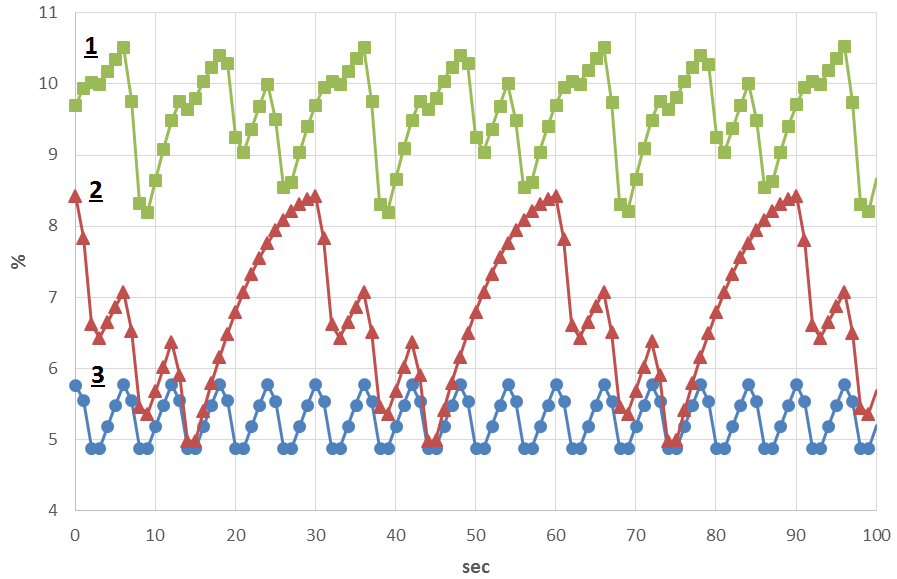
\includegraphics[scale=0.7]{image6}
	\caption{Альвеолярная концентрация $CO_{2} $: 1) Дыхание Биота, 2) дыхание Чейна-Стокса, 3) нормальное дыхание.} 
	\label{image6}
\end{figure}

\begin{figure}[!ht]
	\centering
	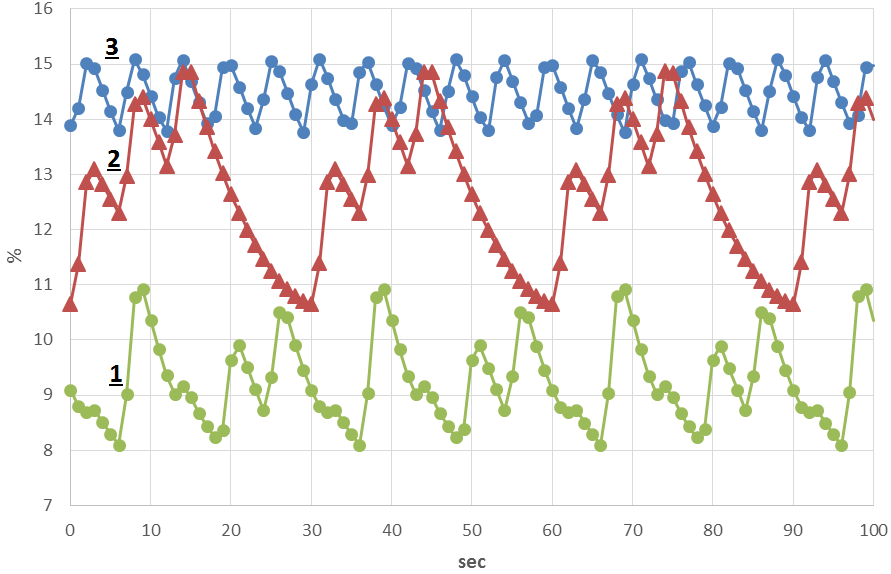
\includegraphics[scale=0.7]{image7}
	\caption{Альвеолярная концентрация $O_{2} $: 1) Дыхание Биота, 2) дыхание Чейна-Стокса, 3) нормальное дыхание.} 
	\label{image7}
\end{figure}

\section{Моделирование альвеолярного газообмена при астме}
Астма - это хроническое воспалительное заболевание дыхательных путей с участием разнообразных клеточных элементов. Ключевое звено бронхиальной астмы любого генеза — повышенная реактивность бронхиального дерева. Она обусловлена нарушением вегетативной регуляции тонуса гладких мышц и действием медиаторов воспаления и приводит к периодической обратимой обструкции бронхов, которая проявляется повышением сопротивления дыхательных путей, перерастяжением лёгких, гипоксемией, вызванной очаговой гиповентиляцией, гипервентиляцией. Несоответствием между вентиляцией и перфузией может привести к увеличению парциального давления $CO_{2} $ и уменьшению парциального давления $O_{2} $ в крови. 

С клинической точки зрения приступы астмы могут быть классифицированы как легкие, умеренные и тяжелые \cite{Colice2004}. В данном разделе приступы астмы моделируются при помощи уменьшения площади поперечного сечения терминальных трубок трахейно-бронхиального дерева $S_{0} $ в уравнении \eqref{GrindEQ__3_}, а также эффективного радиуса альвеолярных объемов $r_{ef} $ в уравнении \eqref{GrindEQ__12_} при помощи зависимости:
\begin{equation} \label{GrindEQ__43_} 
S_{0}^{\gamma } =\pi \left(r_{ef}^{\gamma } \right)^{2} =S_{0}^{norm} {\left(100-\gamma \right)\mathord{\left/ {\vphantom {\left(100-\gamma \right) 100}} \right. \kern-\nulldelimiterspace} 100} ,  
\end{equation} 
где $S_{0}^{\gamma } $, $r_{eff}^{\gamma } $ ~-- модифицированные значения площади поперечного сечения и эффективного радиуса во время приступа астмы; $0\% \le \gamma \le 100\% $ ~-- коэффициент тяжести астмы; $\gamma =0\% $ соответствует нормальным физиологическим условиям; $\gamma =100\% $ соответствует полному схлопыванию терминальных воздушных путей. Результаты численного моделирования показаны на рисунке \ref{image8}.

Значения дыхательного объема и альвеолярной концентрации $O_{2} $ незначительно изменяются при легком приступе астмы ($0\% \le \gamma \le 20\% $), при этом, величина альвеолярной концентрации $CO_{2} $ остается стабильной. Незначительные изменения связаны с наличием резервов кардио-респираторной системы по доставке  $O_{2} $ и выведению  $CO_{2} $. Умеренные приступы астмы ($20\% \le \gamma \le 40\% $) характеризуются заметным уменьшением значения дыхательного объема и альвеолярной концентрации $O_{2} $, а также значительному нарастанию парциального давления $CO_{2} $, ацидоз продолжает прогрессировать. Случай тяжелого приступа астмы ($\gamma >40\% $) характеризуется дальнейшим резким изменением всех описанных выше параметров, которые выходят за физиологические пределы при $\gamma >50\% $. При таком воздействии кардио-респираторная система перестает справляться с поддержанием газообменом на нужном уровне, и без дополнительных воздействий система уже не приходит к состоянию равновесия. Таким образом, верхний предел тяжелого случая астмы, полученный при численном моделировании, находится при значении $\gamma =50\% $.
 
\begin{figure}[!ht]
	\centering
	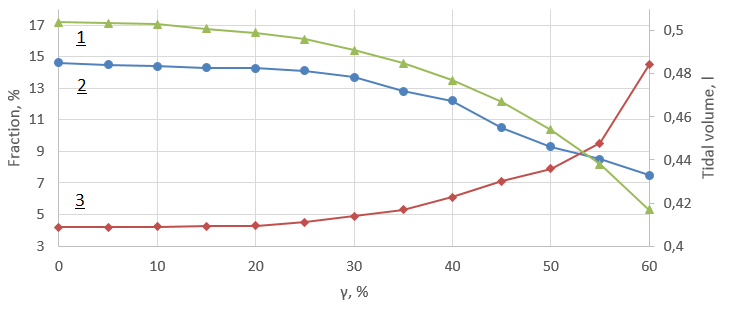
\includegraphics[scale=0.9]{image8}
	\caption{1) Дыхательный объем; 2) Альвеолярная концентрация $O_{2} $; 3) Альвеолярная концентрация $CO_{2} $.} 
	\label{image8}
\end{figure}

\section{Моделирование минутной вентиляции легких в условиях гиперкапнии}
Предложенная модель использовалась для моделирования регуляторного изменения минутной вентиляции легких при дыхании газом с повышенным содержанием $CO_2$ (гиперкапния). С точки зрения спортивной науки рассматриваемое направление исследований представляет большой интерес ввиду того, что респираторная функция является одним из главных лимитирующих факторов организма при интенсивных физических нагрузках характерных для спорта высших достижений. Рассматриваемые в данной работе условия гиперкапнии отчасти воспроизводят широко используемые тренировочные процессы в условиях высокогорья и гипоксии, целью которых является легальное повышение гемоглобина в крови у спортсменов уровня олимпийской сборной.

В работе \cite{reynolds1972} для испытуемых изменяли состав вдыхаемого газа, увеличивая в нем содержание \(CO_{2}\) в интервале от 3\% до 7\%. В соответствии с этим, при численном моделировании проводилось изменение параметра \(C_{CO_{2}}^{air}\). Скорость регуляторного ответа организма регулировалась с помощью параметра \(\tau\) из \eqref{VentReg}. В каждом из случаев его значение 
определялось с помощью линейной регрессии лабораторных данных в логарифмическом масштабе. В результате были получены следующие значения: $\tau_{7\%}=240$~сек., $\tau_{6\%}=220$~сек., $\tau_{3\%}=191$~сек.  


\begin{figure}[!ht]
	\centering
	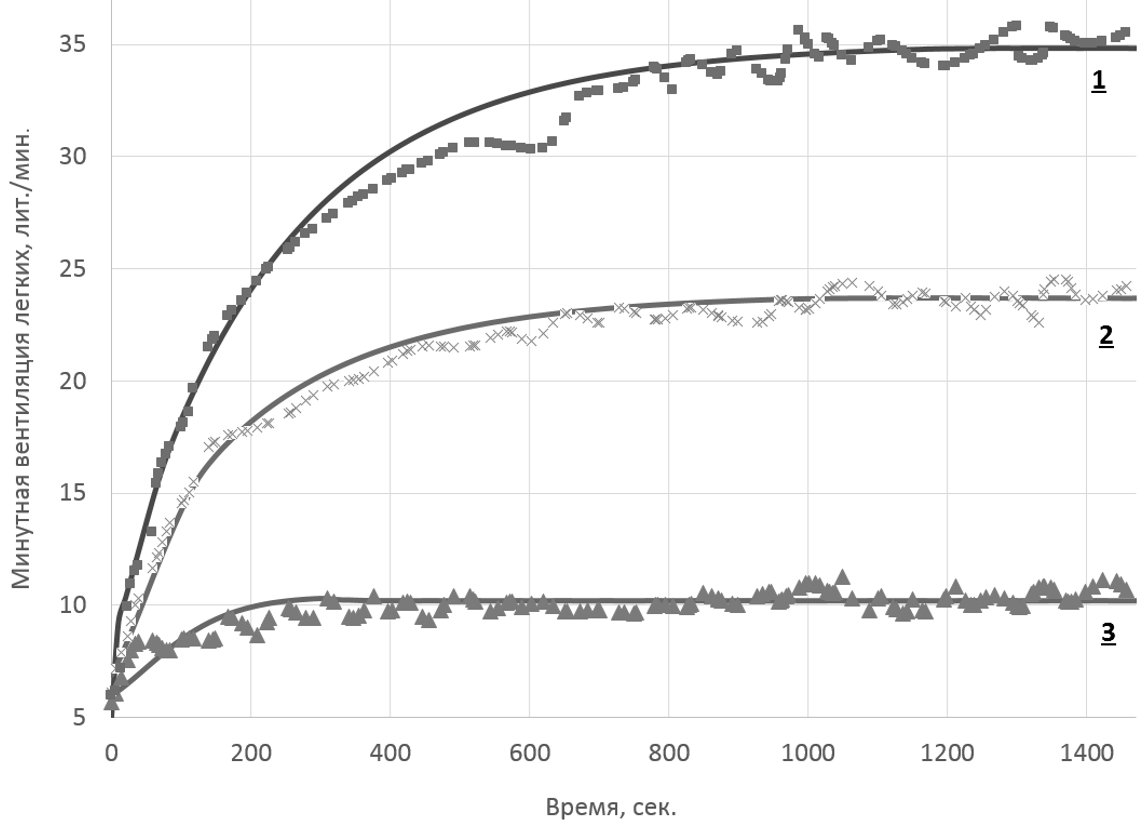
\includegraphics[scale=0.5]{hyper.png}
	\caption{Сравнение изменения минутной вентиляции легких в условиях гиперкапнии при лабораторных исследованиях (приведенные в \cite{reynolds1972} данные обозначены точками) и численном моделировании (данные расчетов обозначены сплошными линиями). 1 ~--- \(7\% \;CO_{2}\), 2 ~--- \(6\% \;CO_{2}\), 3 ~--- \(3\% \;CO_{2}\) } 
\end{figure}

Достигнута высокая степень согласованности между результатами численного моделирования и лабораторных исследований. Для случая гипоксии наблюдались значительные отклонения на начальном этапе эксперимента. Однако, модель позволяет удовлетворительно (в пределах погрешности эксперимента) воспроизвести установившееся значение минутной вентиляции (через $10$~мин. после начала эксперимента).

\section{Тестирование алгоритма определения анаэробного порога}
Рассмотрим пример практического применения алгоритма, взяв реальные данные, полученные во время аэробного тестирования спортсмена на беговой дорожке до отказа. 

Спортсмен: возраст 19 лет, рост 179 см., вес 75.3 кг., имеет 1 сп. разряд. Начальная скорость дорожки составляла 7 км/ч, с последующим увеличением на 0.1 км/ч каждые 10 секунд.

\begin{figure}[!ht]
	\centering
	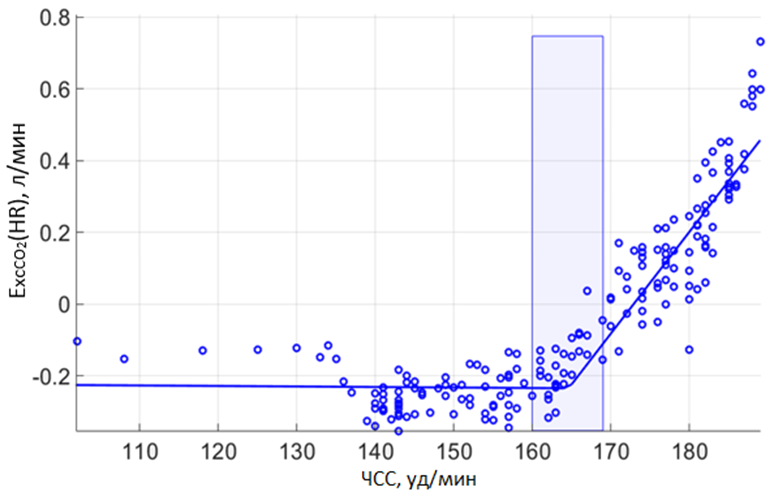
\includegraphics[scale=0.6]{lt1.png}
	\caption{\(Exc_{CO_{2}}\) (дополнительное выделение CO2), ), ПАНО: [160-169] уд/мин.} 
\end{figure}

\begin{figure}[!ht]
	\centering
	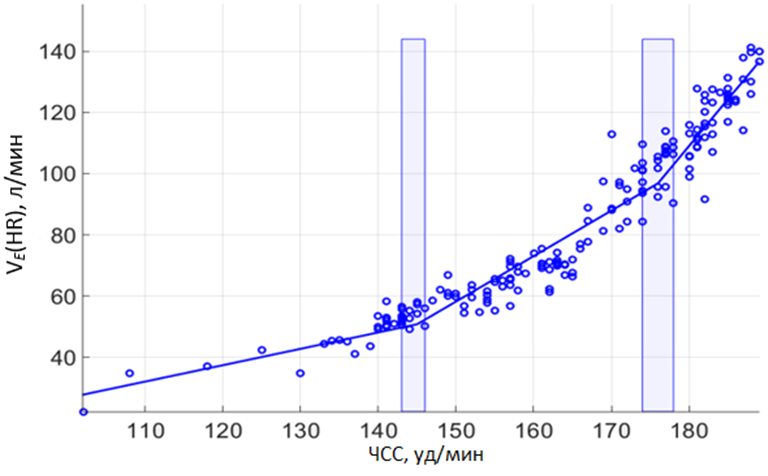
\includegraphics[scale=0.6]{lt2.png}
	\caption{\(V_{E}\) (вентиляция), АэП: [143-146] уд/мин, ПАНО: [174-178] уд/мин} 
\end{figure}

\begin{figure}[!ht]
	\centering
	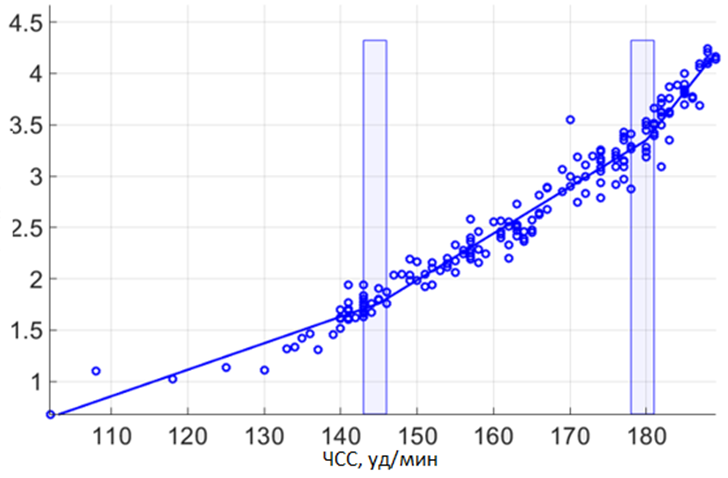
\includegraphics[scale=0.6]{lt3.png}
	\caption{\(V_{CO_{2}}\) (выделение CO2), АэП: [144-146] уд/мин, 
ПАНО: [178-181] уд/мин } 
\end{figure}

\begin{figure}[!ht]
	\centering
	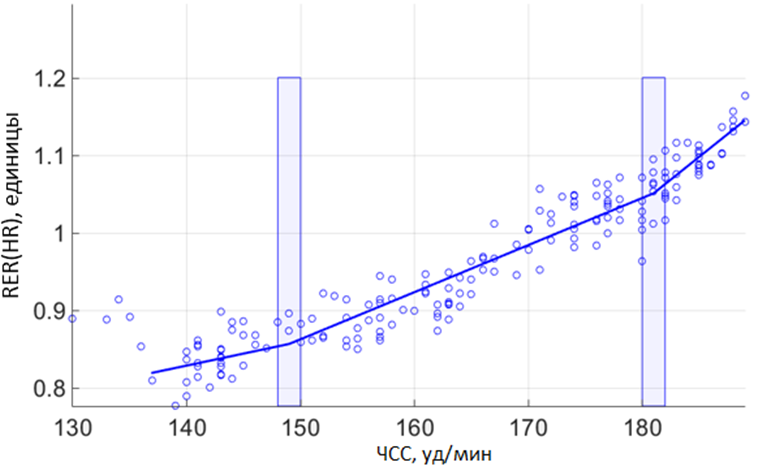
\includegraphics[scale=0.6]{lt4.png}
	\caption{RER (дыхательный эквивалент), АэП: [148-150] уд/мин, 
ПАНО: [180-182] уд/мин} 
\end{figure}

Значения АэП и ПАНО, определенные программным методом близки к оценкам полученным экспертами-физиологами, которые определяют эти значения пользуясь критериями, описанными в \cite{volkov2013} (Таблица \ref{tabular:lt1}). Для интегральной оценки АэП и ПАНО по совокупности критериев можно использовать объединение, пересечение и среднее значение доверительных интервалов (Таблица \ref{tabular:lt2}). Наиболее точным является критерий пересечения интервалов, однако, из-за индивидуальных физиологических особенностей, полученный интервал может быть пустым. Оценка на основе объединения интервалов может оказаться достаточно широкой, поэтому наиболее универсальным способом является средние значения по верхним и нижним границам доверительных интервалов используемых критериев.  

\begin{table}[!ht]
\centering
\caption{Определение АэП и ПАНО по различным критериям}
\medskip
\label{tabular:lt1}
\begin{tabular}{|c|c|c|c|}
\hline
Метод & Параметр & Значение, уд/мин & ДИ 95\%, уд/мин \\
\hline
\(V_{CO_{2}}\) & АэП & 145 & [144-146] \\
\hline
 & ПАНО & 179.5 & [178-181] \\
\hline
\(V_{E}\) & АэП & 144.5 & [143-146] \\
\hline
 & ПАНО & 176 & [174-178] \\
\hline
\(RER\) & АэП & 149 & [148-150] \\
\hline
 & ПАНО & 181 & [180-182] \\
\hline
\(Exc_{CO_{2}}\) & ПАНО & 164.5 & [160-169] \\
\hline
\end{tabular}
\end{table}

\begin{table}[!ht]
\centering
\caption{Определение АэП и ПАНО по различным критериям}
\medskip
\label{tabular:lt2}
\begin{tabular}{|c|c|c|c|c|}
\hline
Метод & Параметр & Эксп. оценка, уд/мин & Ошибка \% & Попадание в ДИ \\
\hline
\(V_{CO_{2}}\) & АэП & 144 & 0.7 & Да \\
\hline
 & ПАНО & 178 & 0.8 & Да \\
\hline
\(V_{E}\) & АэП & 144 & 0.3 & Да \\
\hline
 & ПАНО &  178 & 1.1 & Да \\
\hline
\(RER\) & АэП & 144 & 3.4 & Нет \\
\hline
 & ПАНО & 178 & 1.6 & Нет \\
\hline
\(Exc_{CO_{2}}\) & ПАНО & 178 & 7.5 & Нет \\
\hline
\end{tabular}
\end{table}

\begin{table}[!ht]
\centering
\caption{Определение АэП и ПАНО по совокупности критериев}
\medskip
\label{tabular:lt3}
\begin{tabular}{|c|c|c|}
\hline
Метод & Параметр & Значение параметров, уд/мин \\
\hline
Объединение ДИ & АэП & [143-150] \\
\hline
 & ПАНО & [160-182] \\
\hline
Пересечение ДИ & АэП & Пустое множество \\
\hline
 & ПАНО &  Пустое множество \\
\hline
Среднее значение ДИ & АэП & [145-147.3] \\
\hline
 & ПАНО & [173-177.5] \\
\hline
\end{tabular}
\end{table}

\section{Моделирование тестов с возрастающей нагрузкой в спорте}
\label{sec:loadTests}

Нагрузочные физиологические тесты являются универсальным средством определения индивидуальных параметров работоспособности человека, характеризующих режимы энергообеспечения мышечной деятельности. По этой причине применение таких тестов имеет широкое распространение в спортивной медицине. Эти тесты различаются по своему целевому назначению, применяемым эргометрам и используемым протоколам тестирования. 

\begin{figure}[!ht]
	\centering
	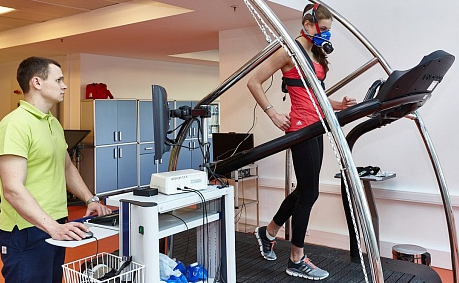
\includegraphics[scale=1.0]{workload.png}
	\caption{Проведение нагрузочного тестирования на беговой дорожке} 
\end{figure}

Для проверки адекватности модели использовались данные, полученные во время аэробного тестирования на беговой дорожке до отказа 10х спортсменов, имеющих 1 сп. разряд и специализирующихся в беге на средние дистанции. 
\begin{table}[!ht]
\centering
\caption{Антропометрические данные спортсменов}
\medskip
\label{tabular:tab1}
\begin{tabular}{|c|c|c|}
\hline
Спортсмен & Рост, m  & Вес, kg \\
\hline
S1 & 1.66 & 61.7 \\
\hline
S2 & 1.80 & 70.8 \\
\hline
S3 & 1.92 & 85.7  \\
\hline
S4 & 1.88 & 73.0  \\
\hline
S5 & 1.71 & 50.9  \\
\hline
S6 & 1.76 & 74.0  \\
\hline
S7 & 1.82 & 70.5  \\
\hline
S8 & 1.85 & 74.6  \\
\hline
S9 & 1.79 & 75.3  \\
\hline
S10 & 1.81 & 71.4  \\
\hline
Avg & 1.80 & 70.8  \\
\hline
\end{tabular}
\end{table}
Начальная скорость дорожки составляла 7км/ч, с последующим увеличением на 0.1 км/ч каждые 10 секунд, наклон дорожки составлял 5 градусов. Газовый состав выдыхаемого воздуха и показатели внешнего дыхания непрерывно определяли прибором “Metamax 3B” (Германия), который калибровали непосредственно перед проведением каждого исследования. Кровь для определения концентрации лактата брали из дистальной фаланги пальца в последние 20 с каждой 3 минуты работы.

В отличии от велоэргометра, мощность выполнения упражнения на беговой дорожке с хорошей точностью рассчитать достаточно сложно, однако можно получить оценку из следующего соотношения:
\begin{equation}
    W=9.8M\vartheta sin(5^{o})
\end{equation}
Где \(\vartheta\)~--- скорость беговой дорожки, M~---масса спортсмена.

Объем легких определялся по формуле \cite{schmidt}:
\begin{equation}
    V=2.5H
\end{equation}
Где H~---рост спортсмена
Общий объем крови \cite{schmidt}:
\begin{equation}
    V_{blood}=77M
\end{equation}

Объем крови в подотделах:
\begin{equation}
    V_{i}=\alpha V_{blood}
\end{equation}
\begin{table}[!ht]
\centering
\caption{Объем крови в подотделах}
\medskip
\label{tabular:blood_volume}
\begin{tabular}{|c|c|}
\hline
\textbf{Отдел} & $\mathbf{\alpha}$ \\
\hline
Системные артерии & 0.252 \\
\hline
Системные вены & 0.64 \\
\hline
Артерии головного мозга & 0.02 \\
\hline
Легочные артерии & 0.048 \\
\hline
Легочные вены & 0.04 \\
\hline
\end{tabular}
\end{table}
Сердечный выброс и распределение кровотока в покое \cite{duke2015,schmidt}:
\begin{equation}
    Q_{SS}=0.187M^{0.81}
\end{equation}
\begin{equation}
    Q_{B,SS}=0.13Q_{SS}
\end{equation}

\begin{table}[!ht]
\centering
\caption{Среднеквадратичные ошибки модели}
\medskip
\label{tabular:tab2}
\begin{tabular}{|c|c|c|c|c|}
\hline
Спортсмен & \(\sigma_{err,O_{2}}\), l/min  & \(\sigma_{err,CO_{2}}\), l/min & \(\sigma_{err,VE}\),  l/min & \(\sigma_{err,LA}\), mmol/l\\
\hline
S1 & 0.05 & 0.07 & 1.22 & 0.11 \\
\hline
S2 & 0.12 & 0.09 & 3.31 & 0.16 \\
\hline
S3 & 0.16 & 0.12 & 4.8 & 0.11  \\
\hline
S4 & 0.11 & 0.11 & 3.3 & 0.29  \\
\hline
S5 & 0.06 & 0.06 & 2.88 & 0.21  \\
\hline
S6 & 0.17 & 0.20 & 8.29 & 0.14  \\
\hline
S7 & 0.11 & 0.11 & 3.51 & 0.05  \\
\hline
S8 & 0.09 & 0.09 & 3.19 & 0.15  \\
\hline
S9 & 0.11 & 0.14 & 5.62 & 0.63  \\
\hline
S10 & 0.12 & 0.11 & 4.35 & 0.07  \\
\hline
\end{tabular}
\end{table}

\begin{table}[!ht]
\centering
\caption{Относительные ошибки модели}
\medskip
\label{tabular:tab3}
\begin{tabular}{|c|c|c|c|c|}
\hline
Спортсмен & \(\sigma_{err,O_{2}}\),\%  & \(\sigma_{err,CO_{2}}\),\% & \(\sigma_{err,VE}\),\% & \(\sigma_{err,LA}\),\%\\
\hline
S1 & 2.3 & 3.5 & 2.5 & 4.8 \\
\hline
S2 & 4.1 & 3.0 & 3.8 & 6.6 \\
\hline
S3 & 4.5 & 3.6 & 3.8 & 4.6  \\
\hline
S4 & 3.2 & 3.7 & 4.3 & 7.2  \\
\hline
S5 & 3.3 & 3.5 & 5.2 & 3.4  \\
\hline
S6 & 6.3 & 7.1 & 10.3 & 4.6  \\
\hline
S7 & 3.5 & 4.0 & 4.3 & 3.3  \\
\hline
S8 & 3.1 & 2.9 & 3.9 & 9.0  \\
\hline
S9 & 3.6 & 4.7 & 6.6 & 12.2  \\
\hline
S10 & 4.5 & 4.3 & 5.9 & 3.4  \\
\hline
Avg & 4.3 & 4.5 & 5.4 & 6.4  \\
\hline
\end{tabular}
\end{table}

\begin{table}[!ht]
\centering
\caption{Параметры модели мышечного метаболизма}
\medskip
\label{tabular:tab4}
\begin{tabular}{|c|c|c|c|c|c|}
\hline
 & \(e_{a}\), кДж/l & \(u_{la}\), $10^{-3}$ $c^{-1}$ & \(\kappa_{CO_{2}}\), $c^{-1}$ & $\beta$, $10^{-2}$ & \ $\alpha$, $10^{-2}$ \\
\hline 
S1 & 4.87$\pm$0.05 & 1.6$\pm$0.18 & 3.78$\pm$0.54 & 1.92$\pm$0.04 & 7.88$\pm$0.18   \\  \hline 
S2 & 4.42$\pm$0.07 & 0.88$\pm$0.09 & 2.11$\pm$0.55 & 0.8$\pm$0.02 & 7.3$\pm$0.04   \\  \hline 
S3 & 3.96$\pm$0.04 & 1.4$\pm$0.07 & 1.79$\pm$0.52 & 1.32$\pm$0.02 & 9.8$\pm$0.11   \\  \hline 
S4 & 3.92$\pm$0.06 & 1.23$\pm$0.1 & 1.63$\pm$0.26 & 0.7$\pm$0.01 & 6.62$\pm$0.1   \\  \hline 
S5 & 4.88$\pm$0.02 & 1.25$\pm$0.12 & 2.02$\pm$0.04 & 1.6$\pm$0.02 & 10.36$\pm$0.08   \\  \hline 
S6 & 4.97$\pm$0.03 & 1.75$\pm$0.06 & 7.04$\pm$0.38 & 0.69$\pm$0.0 & 7.6$\pm$0.02   \\  \hline 
S7 & 4.08$\pm$0.04 & 1.66$\pm$0.28 & 2.66$\pm$0.18 & 0.4$\pm$0.01 & 8.84$\pm$0.02   \\  \hline 
S8 & 4.94$\pm$0.02 & 5.42$\pm$0.97 & 4.87$\pm$0.28 & 2.29$\pm$0.16 & 3.97$\pm$0.03   \\  \hline 
S9 & 4.69$\pm$0.09 & 8.75$\pm$0.73 & 1.45$\pm$0.19 & 4.58$\pm$0.2 & 3.91$\pm$0.01   \\  \hline
S10 & 4.71$\pm$0.09 & 2.03$\pm$0.1 & 4.81$\pm$0.58 & 1.1$\pm$0.02 & 7.75$\pm$0.05   \\  
\hline 
\end{tabular}
\end{table}


С помощью численной расчетов был подобраны параметры модели мышечного метаболизма.

Полученные оценки КПД согласуются с физиологически обоснованными значениями. Однако, полученные значения нельзя считать истинной оценкой КПД, а только неким аналогом в силу грубости оценки мощности упражнения, а также не учета в модели того факта, что часть лактата используется как энергетический субстрат окисления (в экспериментальных работах измерение КПД производится при нагрузка меньше величины порога анаэробного обмена).

Значения параметра \(u_{la}\), характеризующего скорость утилизации лактата, получились близки к экспериментальным данным, свидетельствующим, что восстановление уровня лактата к исходному происходит примерно через 60-90 минут после окончания нагрузки. 

Экспериментальные данные, по которым производилась идентификация параметров модели, очень сильно зашумлены. Это связанно как с погрешностью измерительных приборов, так и с особенностями адаптации организма к физической нагрузке (у более квалифицированных спортсменов дисперсия точек заметно меньше, т.к. их организм привык к нагрузкам и врабатываниые происходит более направленно). Присутствует погрешность численного метода решение ОДУ, а также алгоритм стохастической оптимизации может приводить к различным результатам. Поэтому для оценивания параметров модели использовался статистический метод бутсреппинга, на основе результатов которого рассчитывалась дисперсия.     
В результате было получено, что для \(e_{a}\) дисперсия составляет примерно 1.1\%, для \(u_{la}\)~--- 9.6\%, для \(\kappa_{CO_{2}}\)~--- 12.9\%, для \(\beta\)~--- 2.5\%, для \(\alpha\)~--- 1\%..


\begin{table}[!ht]
\centering
\caption{КПД выполнения упражнения}
\medskip
\label{tabular:tab5}
\begin{tabular}{|c|c|c|c|}
\hline
Спортсмен &  \(\eta\), \% & Спортсмен &  \(\eta\), \% \\
\hline
S1 & 23.3$\pm$0.2 & S6 & 24.1$\pm$0.1\\
\hline
S2 & 22.0$\pm$0.3 & S7 & 19.9$\pm$0.2\\
\hline
S3 & 19.4$\pm$0.2 & S8 & 24.2$\pm$0.1\\
\hline
S4 & 19.0$\pm$0.3 & S9 & 22.9$\pm$0.4\\
\hline
S5 & 23.5$\pm$0.1 & S10 & 22.8$\pm$0.4\\
\hline
\end{tabular}
\end{table}

При выполнении физического упражнения первые несколько движений осуществляются за счет внутримышечных запасов АТФ, которые быстро заканчиваются, в следующие 10-60 сек основным источником энергии является креатинфосфат. В модели данные механизмы не учитываются, поэтому на начальных участках графиков потребления кислорода и выделения углекислого газа присутствует заметное расхождение. Ошибка лактатной кривой объясняется упрощением модели: не рассматриваются отдельно различные процессы утилизации лактата в мышцах, миокарде, в печени и кишечнике в результате глюконеогенеза, вклад отдельных буферных систем крови (в том числе индивидуальные емкости), очень простое представление об образовании лактата и поступлении его в кровь, а также особенностями получения экспериментальных данных.


\clearpage
\section{Резюме}
\begin{itemize}
\item 
Выполнена проверка адекватности 0D-1D модели дыхательной системы. После подбора параметров в физиологических пределах, модель показала хорошее совпадение альвеолярного потока и альвеолярного давления в нормальных условиях с литературными данными.
\item 
Выполнен поиск оптимальной чистоты(обеспечивающей наилучший газообмен) ИВЛ. Полученное значение(0.17 Hz) находится достаточно близко к экспериментально измеренной величине чистоты дыхания пациента в нормальном состоянии(0.23 Hz).
\item
Выполнено моделирование патологических рисунков дыхания: дыхание Биота и Чейна-Стокса. Сравнение с нормальным синусоидальным дыханием подтвердило, что при наличии патологии газообмен становится менее эффективным. 
\item
Выполнено моделирование легких, умеренных и тяжелых приступов астмы. Определены параметры, соответствующие каждому типу приступа. Результаты качественно совпали с описанием из клинической литературы, к сожалению не удалось найти количественные значения, с которыми можно было бы провести сравнение.
\item
Выполнено моделирование минутной вентиляции легких в условиях гиперкапнии. Достигнута высокая степень согласованности между результатами численного моделирования и лабораторных исследований. Модель позволяет удовлетворительно воспроизвести установившееся значение минутной вентиляции. 
\item
Протестирован алгоритм определения аэробного и анаэробного порогов по нескольким физиологическим показателям. Алгоритм показал хорошую согласованность с оценками эксперта-физиолога.
\item 
По результатам тестов с возрастающей нагрузкой для десяти спортсменов была выполнена идентификации параметров модели мышечного метаболизма. Для части параметров дисперсия (оценена методом бутстреппинга) получилась достаточна большой, а для других не превышала 5\%. Тем не менее модель показала хорошее совпадение с экспериментом


\end{itemize}